% generated by scripts/pkl_to_latex.py
% source PKL : uscan_v1_L6_Ne4_t1_mode-uniform_nmin2_solver-gcg_sz0_restarts10_iter300_kmax4_tol1em09_U1to20_N20-d03a74da789e.pkl
% scan type  : uscan
% state      : gs
% requires   : \usepackage{pgfplots} \pgfplotsset{compat=1.18}
% colours match the matplotlib PDF (tab10 cycle)
\definecolor{gmeC0}{HTML}{1F77B4}
\definecolor{gmeC1}{HTML}{FF7F0E}
\definecolor{gmeC2}{HTML}{2CA02C}
\definecolor{gmeC3}{HTML}{D62728}
\definecolor{gmeC4}{HTML}{9467BD}
\definecolor{gmeC5}{HTML}{8C564B}
\definecolor{gmeC6}{HTML}{E377C2}
\definecolor{gmeC7}{HTML}{17BECF}

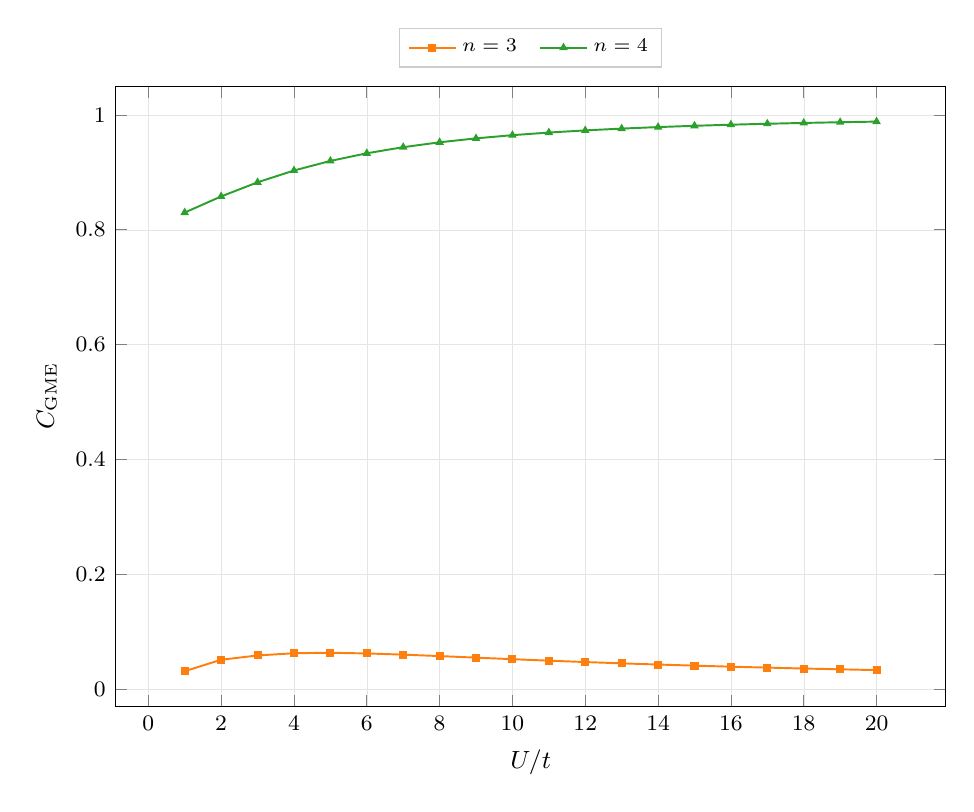
\begin{tikzpicture}
  \begin{axis}[
    width=\columnwidth,
    height=0.78\columnwidth,
    xlabel={$U/t$},
    ylabel={$C_{\mathrm{GME}}$},
    grid=both,
    grid style={line width=.1pt, draw=gray!20},
    tick label style={font=\footnotesize\rmfamily, /pgf/number format/fixed},
    label style={font=\small\rmfamily},
    scaled ticks=false,
    legend style={font=\scriptsize\rmfamily, draw=gray!40, at={(0.5,1.03)}, anchor=south, /tikz/every even column/.append style={column sep=6pt}},
    legend cell align={left},
    legend columns=2,
    ymin=-0.03,
    ymax=1.05,
  ]
    \addplot[color=gmeC1, mark=square*, mark size=1.1pt, line width=0.7pt] coordinates {
        (1,0.031216) (2,0.051105) (3,0.058563) (4,0.062507)
        (5,0.063276) (6,0.062116) (7,0.06002) (8,0.057521)
        (9,0.054782) (10,0.052128) (11,0.049516) (12,0.047114)
        (13,0.044869) (14,0.04277) (15,0.040851) (16,0.039068)
        (17,0.037418) (18,0.035843) (19,0.034433) (20,0.033102)
    };
    \addlegendentry{$n=3$}
    \addplot[color=gmeC2, mark=triangle*, mark size=1.1pt, line width=0.7pt] coordinates {
        (1,0.82987) (2,0.857939) (3,0.882552) (4,0.903102)
        (5,0.919767) (6,0.9331) (7,0.943732) (8,0.952237)
        (9,0.959083) (10,0.964641) (11,0.969193) (12,0.972955)
        (13,0.976092) (14,0.97873) (15,0.980966) (16,0.982875)
        (17,0.984517) (18,0.985938) (19,0.987176) (20,0.988259)
    };
    \addlegendentry{$n=4$}
  \end{axis}
\end{tikzpicture}
